\documentclass[12pt]{article}
\usepackage[margin=3.0cm]{geometry}
\usepackage[french, english]{babel}
\usepackage[utf8]{inputenc}
\usepackage{graphicx}
%\usepackage[hidelinks]{hyperref}
\usepackage{amsmath}
\graphicspath{{Images/}
\geometry{legalpaper}}

\begin{document}
\begin{titlepage} 
	\large
	{
		\begin{center}
			UNIVERSITÉ DE SHERBROOKE\\Faculté de génie\\
			Département de génie électrique et génie informatique\\
			\vspace{3cm}
			{\LARGE\textbf{Principes de dynamique et méthodes numériques}}\\
			\vspace{2cm}
			\LARGE{Rapport APP2}\\
			\vspace{2cm}
			Présenté à\\l'équipe professorale de la session S4\\
			\vspace{2cm}
			Produit par\\Axel Bosco, Jacob Fontaine, Philippe Spino\\
			\vspace{1cm}
			\vfill{23 mai 2017 - Sherbrooke}
		\end{center}
	}
\end{titlepage}
\tableofcontents
\newpage
\section{Introduction}
Principes de dynamique et méthodes numériques
Dans le cadre du cour \textit{Principes de dynamique et méthodes numériques}, le mandat remit à la présente équipe était de rendre l'initiation des étudiants de la faculté de génie plus passionnante a l'aide d'un parcours à obstacles de style \textit{Wipe-out}.

\section{Design de la glissade}
Le devis émit par le WOQ demandais de calculer la trajectoire d'un glissade passant absolument par des points cartésiens précis. Comme le montre la tableau 1, la glissade doit passer par tout les points.

\begin{center}
	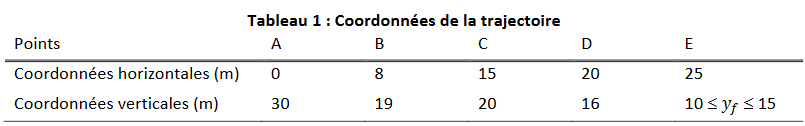
\includegraphics[scale=0.8]{tableau1}
\end{center}
Les valeurs de ce tableau sont les points de référence pour le approximation de la courbe de la glissade. Il faut approximer une courbe qui passe par tous les points. Ensuite, il faut trouver la bonne courbe en évaluant toutes les courbes possibles des points $E_y$. Les valeurs possibles du points $E_y$ vont de 10 à 15. Les coordonnées horizontales$(m)$ sont exprimés par la suite $X_k$ et les coordonnées verticales$(m)$ sont exprimées par la suite $Y_k$. 
\subsection{Calculs}
Il y a 5 termes par suites mentionnés précédemment. Le devis demander d'interpoler les valeurs des coordonnées. L'interpolation veut dire que notre nombre de termes dans les suites, soit M, est égale au nombre de termes du polynôme, soit $N=M$. En utilisant l'appoximation linéaire, on obtien un polynome d'ordre 4 (l'ordre est $N-1$). Le polynôme obtenu suite a l'interpolation est: 
\begin{equation}
g(x) = A(1) + A(2)\times x + A(3)\times x^2 + A(4)\times x^3 + A(5)\times x^4 
\end{equation}
Ou $A$ est le vecteur des coefficient des polynômes obtenu par la méthode de la projection orthogonale avec la pseudo-inverse. 
\newpage
\noindent
Une fois les polynômes trouver ($E_y$ allant de 10 à 15 par bon de 0,01), il faut choisir une des courbe qui assure la sécurité des participants. Le devis mention que: "La valeur de yf doit assurer une sortie de glissade à peu près horizontale (exigence qualitative) pour assurer une transition naturelle avec la surface horizontale de la trappe." On peut alors dire qu'il faut que la dérivé du polynôme soit le plus près de 0. 
\begin{equation}
\frac{dg(x)}{dx} = 0
\end{equation}
L'estimation a été accomplie avec le logiciel de calcul Matlab et le résultat obtenu est que la valeur de $E_y = 12.27m$. 

\section{Design du débit d'eau}
\subsection{Calculs}

\section{Design du Ballon-mousse}
\subsection{Ballon Attrapé}
Dans cette situation, on présume que le participant attrape le ballon-mousse. Donc, on peut assumer alors qu'il y a une fusion du ballon-mousse et le participant après l'impacte en ceux-ci? Donc cela se résume à l'équation suivante:
\begin{equation}
m_p\times v_p + m_b\times v_b = (m_p + m_b)\times v_{pb}
\end{equation}
En isolant $v_{pb}$, on obtien un valeur de :
\begin{equation}
v_{pb} = 5,59m/s
\end{equation}
À l'aide de cette vitesse, on doit règler la minutrie en sorte à ce que le participant ait quitté la plateform au complet avant que celle-ci s'ouvre.
\begin{equation}
\delta t_m = \frac{l_{trappe}}{v_{pb}}
\end{equation}
\begin{equation}
\delta t_m = \frac{3m}{5,59m/s} \approx{0,54}
\end{equation}
Et selon les standard imposés, la minutrie devait avoir une marge de manoeuvre de $0,02s$.
\begin{equation}
\delta t_m \approx{0,54 - 0,02} = 0,52sec
\end{equation}
\subsection{Ballon non attrapé}
Dans cette situation, le participant entre en collision avec le ballon sans l'attrapé. La collision entre le ballon-mousse et le participant à ce moment là est une collision plastique. Selon les requis du devis de WOQ, nous considérons le coefficient de récupération de $0,8$. Les valeurs de $V_{p_n}$ = 6.25$m/s$ et $V_{b_n}$ = -1.0$m/s$
\begin{equation}
e <= 0,8 = \frac{V'_{b_n} - V'_{p_n}}{V_{p_n} - V_{b_n}}
\end{equation}
suite a des manipulations algébrique, le résultat est:
\begin{equation}
{V_{b_n} - V_{p_n}} = 5,8
\end{equation}
\begin{equation}
V_b' = 5,8 + V_p'
\end{equation}
Il y a aussi l'équation suivante:
\begin{equation}
m_p\times V_p + m_b\times V_b = m_p\times V_p' + m_b\times V_b'
\end{equation}
\noindent
en substituant l'équation trouvé précédement, on obtien:
\begin{equation}
V_p' = \frac{m_p.V_p + m_b.V_b}{(m_b + m_p).V_b'}
\end{equation}
\begin{equation}
V_p' = 5.06m/s
\end{equation}
Donc, le temps requis pour traverser complètement la trappe est:
\begin{equation}
t_m = \frac{l_{trappe}}{V_p'} = 0,59 sec
\end{equation}

\section{Design de la minuterie}
Le devis avait un requis d'une marge de maneuvre de $0,02sec$ pour assurer la sécurité des participants concernant la trappe. Lorsque le ballon est attrapé, les temps est de $0,52sec$ et lorsque le ballon rebondit, le temps est de $0,59sec$.
\subsection{Calculs}
\begin{equation}
t_{m_f} < \Delta T_m - 0,02
\end{equation}
\begin{center}
et
\end{center}
\begin{equation}
t_{m_r} > \Delta T_m + 0,02
\end{equation}

Suite aux manipulations algébriques, le résultat est que 
\begin{equation}
\Delta T_m \approx 0,056 sec
\end{equation}

\section{Design du Coussin-Tampoline}
En ce qui concerne le design du Coussin-Trampoline, le devis fournit toutes les informations nécessaires pour déterminer la déformation totale du coussin-trampoline. Sachant que $k_c = 6000N/m$ et que le participant-ballon, d'une masse de $m = 88kg$ tombe d'une hauteur $h_0$ de $5 m$. Sachant que le coussin va avoir une déformation de $h_c$, la chute totale du participant-ballon est de $\Delta h = h_0 + h_c$. La vitesse horizontale du participant-ballon n'affecte pas sa vitesse verticale, seule la gravité va affecter sa vitesse.
\subsection{Calculs}
Sachant que,
\begin{equation}
T_i + V_{gi} + V_{ri} = T_f + V_{gf} + V_{rf}
\end{equation}
Où,
\begin{equation}
T_i = 0
\end{equation}
\begin{equation}
V_{ri} = 0
\end{equation}
\begin{equation}
T_f = 0
\end{equation}
\newline
Au début de la chute, la vitesse verticale du participant-ballon est nulle. À la fin de la chute, la vitesse verticale du participant est nulle, puisque le coussin-trampoline a amorti la chute. Aussi, la déformation du coussin-trampoline est nulle, donc il n'y a aucune énergie potentielle de ressort. 
\newline
\newline
Donc, le théorème d'énergie mécanique après simplification devient,
\begin{equation}
V_{gi} = V_{gf} + V_{rf} 
\end{equation}
Sachant que,
\begin{equation}
V_{gi} = m \times g \times h_0 
\end{equation}
\begin{equation}
V_{gf} = m \times g \times h_c 
\end{equation}
\begin{equation}
V_{rf} = \frac{1}{2} \times k_c \times h_c^2
\end{equation}
\newline
En substituant les équations de chacun des composants du théorème, l'équation devient,
\begin{equation}
m \times g \times h_0 = m \times g \times h_c + \frac{1}{2} \times k_c \times h_c^2
\end{equation}
\newline
\newline
Il est possible de transformer cette équation en équation quadratique.
\begin{equation}
0 = \frac{1}{2} \times k_c \times h_c^2 + m \times g \times h_c - m \times g \times h_0
\end{equation}
\newline
En résolvant l'équation quadratique, la valeur de $h_c$ est obtenue.
\subsection{Résultats}
La résolution d'une quadratique donne deux valeurs. Les deux valeurs obtenues sont affichées ci-bas.
\begin{center}
	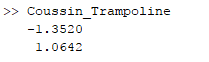
\includegraphics[scale=0.8]{valeurhc}
\end{center}
Puisqu'il s'agit d'une compression d'un ressort, la valeur de la distance de compression doit être négative. Donc, la valeur de $h_c = -1,3520m$.
\section{Design du Bassin}
\subsection{Calculs}

\section{Conclusion}


\end{document}